\documentclass[12pt,a4paper]{article}
\usepackage{tabularx}
\usepackage{booktabs}
\usepackage{longtable}
\usepackage{ltxtable}
\usepackage[latin1]{inputenc}
\usepackage{amssymb}
\usepackage[]{graphicx,rotating}
\usepackage[T1]{fontenc}
\usepackage{parskip}
\usepackage{listings}
\usepackage{natbib}
\usepackage[official]{eurosym}
\usepackage{mathrsfs}
\usepackage{amsmath}
\usepackage{verbatim}
\usepackage[usenames,dvipsnames]{color}     %for R colors and formatting
\usepackage[font=small,labelfont=bf,format=hang]{caption} %makes Figure/Table/Listing bold and decreases size of caption
\usepackage[left=3cm, right=2.5cm, top=2.5cm]{geometry}

\pagestyle{empty}
\parindent 0cm
\renewcommand{\baselinestretch}{1}
\newcommand{\bs}{\boldsymbol}
\renewcommand{\familydefault}{cmr}
\pdfminorversion=7
\bibliographystyle{agsm}

\lstset{ %for R colors and formatting
  language=R,                     % the language of the code
  basicstyle=\scriptsize\ttfamily, % the size of the fonts that are used for the code
  numbers=left,                   % where to put the line-numbers
  numberstyle=\scriptsize\color{Blue},  % the style that is used for the line-numbers
  stepnumber=1,                   % the step between two line-numbers. If it is 1, each line
                                  % will be numbered
  numbersep=5pt,                  % how far the line-numbers are from the code
  backgroundcolor=\color{white},  % choose the background color. You must add \usepackage{color}
  showspaces=false,               % show spaces adding particular underscores
  showstringspaces=false,         % underline spaces within strings
  showtabs=false,                 % show tabs within strings adding particular underscores
  frame=single,                   % adds a frame around the code
  rulecolor=\color{black},        % if not set, the frame-color may be changed on line-breaks within not-black text (e.g. comments (green here))
  tabsize=2,                      % sets default tabsize to 2 spaces
  %captionpos=b,                   % sets the caption-position to bottom
  breaklines=true,                % sets automatic line breaking
  breakatwhitespace=false,        % sets if automatic breaks should only happen at whitespace
  keywordstyle=\color{RoyalBlue},      % keyword style
  commentstyle=\color{YellowGreen},   % comment style
  stringstyle=\color{ForestGreen}      % string literal style
} 


\begin{document}

\begin{center}
% \vspace*{1cm}
 
\includegraphics[width=0.35\textwidth]{GU-Logo-blau-CMYK.eps} \vspace{2cm}

 {\Large{\bf Bayesian Beer Market Estimation}} \medskip

  {\Large{Simulating Nash Equilibrium Market Outcomes with Bayesian Analysis of Choice-Based Conjoint Data}} \vspace{3cm}  
 
  by \medskip

  \textbf{Sourangshu Ghosh} \\
  
  July 21, 2019
  
\end{center}


\pagebreak
\pagestyle{plain}
\pagenumbering{Roman}
\tableofcontents
\pagebreak
\listoffigures
%\pagebreak
\listoftables
%\newpage
\renewcommand\lstlistlistingname{List of R Code Chunks}
\lstlistoflistings
\newpage
\setcounter{page}{2}
\pagenumbering{arabic}
\setlength{\baselineskip}{1.5\baselineskip}
\pagestyle{plain}


\section{Introduction and a Primer on the Beer Market} \label{sec_intro}
Which beer would Thomas Bayes, the famous philosopher and statistician that first described Bayes' Theorem \citep{bayesEssaySolvingProblem1763} prefer?
Though a particular preference by Bayes for a certain product cannot be inferred and this question remains unanswered by the present study, modern Bayesian methods provide a sophisticated way to estimate today's customers' individual preferences based on their choices.
This paper uses Bayesian methods applied on choice-based conjoint (CBC) data to simulate Nash equilibrium market outcomes in the beer market.
The remainder is structured as follows: First, this section introduces the beer market and the assumptions necessary for further analysis.
Then, section \ref{sec_motivation} motivates the analytical model, while chapter \ref{sec_vars_relat} introduces the data set and hypothesizes the expected relationships between the market simulation metrics.
The paper then introduces the heterogeneous MNL model with BLP-type indirect utilities and presents its results (section \ref{sec_model}), followed by a discussion of the resulting beer market simulation.
The last section concludes by discussing managerial and research implications that can be derived from the present analysis.

The leading international breweries today face the challenges of decreasing beer consumption in Europe, new trends such as craft beer and increased regulatory pressure \citep{jpmorganWhatTapGlobal2018}.
The second largest brewery worldwide after Anheuser-Bush InBev is Heineken, owning more than 300 brands including well-known ones such as Amstel \citep{heinekenHeinekenAnnualReport2019}.
To counter the threads by the aforementioned trends, Heineken can merge with other beer brands to incrementally increase their profits through leveraging higher price setting power due to market consolidation.
Though Heineken already acquired Amstel in 1968 \citep[p. 49]{oliverOxfordCompanionBeer2011}, this paper looks at the merger from today's perspective.
The goal of this research is to assess whether a merger of Heineken and Amstel, based on today's customer preferences and market conditions would still be considered beneficial.
Towards this end, the present study subsequently derives the producer surplus of Heineken and Amstel before and after the merger and compares that to a potential merger of Heineken with another national brand, Estrella.

\section{The Necessity of Enhancing the Standard MNL Model} \label{sec_motivation}
Historically, marketing research has heavily relied on Conjoint Analysis as a tool to measure consumers' preferences by asking them to choose between different products that imply trade-offs \citep{greenConjointAnalysisMarketing1990}.
This is a method to derive consumers' preferences in a more credible way than to ask them which brand or feature they prefer,
since this often yields trivial results\footnote{i.e. preferring the cheap vs. the expensive good or valuing the better quality good more than the low quality product.}.
Choice-based conjoint data enables researchers to calculate counterfactual scenarios, such as what happens to a company's market share if a competitor changes its price \citep{huberDealingProductSimilarity2001}.
To analyze choice-based conjoint data, market research has focused on the Multinomial Logit (MNL) Model.
Unfortunately, the MNL model is based on two strong and unrealistic assumptions \citep{elrodEmpiricalComparisonRatingsBased1992}.
First, choices should be independent of irrelevant alternatives (IIA).
This means that consumer's choices are not influenced by the presence or absence of another, supposedly irrelevant other choice option.
However, numerous examples have been constructed to easily show that this assumption is often violated, most famously the blue and red bus example by \cite{mcfaddenConditionalLogitAnalysis1973}.
Especially for substitute products, this assumtion therefore does not hold. 
Modeling very similar choices with a traditional MNL model is hence not desirable.
The second strong assumption that is required for MNL estimation is homogeneity in preferences across consumers.
This implies that consumer's preferences---expressed by the beta coefficients---are identical for all consumers, which does not hold in reality. Literature has acknowledged those violations and proposed the heterogeneous MNL, a more flexible model that relaxes the IIA assumption and allows for differences in preferences by modeling individual MNL models for every single customer \citep{steckelHeterogeneousConditionalLogit1988}.

When taking the beta coefficients from this hierarchical MNL model to simulate individual choices as well as aggregate market outcomes and equilibrium prices,
the standard approach was to assume that all prices in the choice set were within the consumer's unobserved budget.
\cite{pachaliPerilsIgnoringBudget2017} argue that this simplification can lead to a serious over-estimation of equilibrium prices.
They claim that this is still the case if priors such as sign constraints are included and reasonably specified in the estimation as by \cite{sonnierHeterogeneityDistributionsWillingnesstopay2007} and \cite{allenbyEconomicValuationProduct2014}.
Instead of manipulating the data a priori until derived estimates mirror the desired price ranges, this paper follows \cite{pachaliPerilsIgnoringBudget2017}
and applies a model specification which is capable of inferring previously unobserved budgets additionally to sign constraints for $\beta_{price}$.
To that matter, the present study implements the indirect utility model by \cite{berryAutomobilePricesMarket1995}.
It is superior to the price screening model proposed by \cite{gilbrideChoiceModelConjunctive2004},
since it models a continuous choice probability dependent on price.
Logit choice probabilities need to be continuous at every draw in order to derive a pure-strategy Nash equilibrium \citep{morrowFixedPointApproachesComputing2011a, pachaliPerilsIgnoringBudget2017}.

Concluding this section, the analytical model implemented in this study addresses three serious shortcomings of most common methods to conduct a market simulation and derive profit-maximizing prices.
It relaxes the IIA assumption, allows for heterogeneous individual-level consumer preferences, and infers unobserved budgets.
Those three model specifications are believed to yield more realistic and less biased estimates \citep{chandukalaChoiceModelsMarketing2008, pachaliPerilsIgnoringBudget2017}.


\section{Exogenous Variables and Expected Relationships} \label{sec_vars_relat}

While the previous section motivated the analytical model and presented model extensions to relax unrealistic assumptions,
this part introduces the empirical application of those tools.
This paper analyzes a choice-based conjoint data set for choices among different beer brands obtained by the market research institute Kantar TNS.
The data set recorded preferences for canned beer presumably in the Spanish market.
 $N=407$ respondents participated in the study and chose among $p=10$ alternatives per choice task (nine beer brands and one outside option).
Every participant performed $t=15$ choice tasks. In total, 15 distinct beer brands and one outside alternative were included in the study,
while the subjects were only presented with a subset of $p$ alternatives, always including the outside alternative (i.e. no purchase).
The data set consists multiple brands of the same brewery---four Amstel beers and two Estrella and Mahou beers each.
The remaining seven beer brands based on their brand names are assumed to belong to different companies.
Additionally to the brand names, the price was displayed to the subjects, which ranged from 0.22 to 0.74\text{ \euro }.

Consistent with economic theory, there should be a negative relationship between price and demand.
The less competition and hence more market power is present, the higher should be the prices, which should come with less demand for beer.
Demand is measured in relative market share in this model, which means a decrease in the inside goods' shares should come with an increase in the outside option's share (i.e. more consumers drop out of the market and do not purchase any product).
Besides price and market share, profit is the most important metric that is optimized by the individual players in the market.
Though there is a clear intuition how prices and market shares develop dependent on the competitive scenario, no trivial statement can be made about profits.
With higher prices comes usually a lower market share---thus we cannot tell a priori which effect should have a stronger impact on profits.
To come up with an estimate for profits, this study assumes constant marginal costs of 0.192\text{ \euro } per 0.33~cl can across all producers.
This estimation is based on Heineken's costs reported in the 2018 annual report \citep{heinekenHeinekenAnnualReport2019}. 
The author assumes the data set to be ten years old, hence the 2018 variable costs are discounted by the compounded average inflation rate of the last decade.
Since standard beer consists of the same ingredients and the degree of economies of scale is assumed to not differ significantly between the considered subset of large breweries, Heineken's marginal costs are assumed to be a good approximation for all other brands' marginal costs.

Profit will then be used to calculate the producer surplus before and after the Heineken--Amstel merger.
This metric enables an assessment whether there is any incremental profit to this transaction.
Since the preferences for Heineken and Amstel are most similar\footnote{see section \ref{sec_model} for the beta coefficients of the individual brands and their interpretation} in the considered subset of the market, the expected incremental profit of a merger between Heineken and Amstel should be higher than the sum of individual profits of a merger between brands that have less correlated preferences, such as Heineken and Estrella.
While the next section introduces the underlying analytical model and its result, detailed market simulation outcomes are discussed in section \ref{sec_marketsim}.


\section{Model Description and Results} \label{sec_model}

Based on the motivation for the analytical model described in section \ref{sec_motivation}, this section first discusses the implemented model and then presents its results.
This study uses a heterogeneous MNL model and utilizes Bayesian methods to generate the individual-level beta coefficients and the specification of the prior distribution.
One of the assumptions of the standard MNL model is homogeneity in preferences across all consumers.
To allow for different preferences, every consumer needs to be described by an individual MNL model.
However, since every participant only recorded $t=15$ choice tasks, there are not enough observations to reliably estimate such a model.
That is why this study uses Bayesian estimation with the Markov Chain Monte Carlo (MCMC) routine to sample the individual-level betas and estimate the parameters for the prior distribution.

The resulting beta coefficients are a measure of customer preferences---a greater beta translates to a higher preference for a product, while a negative value implies dis-utility from that good for the consumer.
The distribution of betas can then be used to compute market shares either based on posterior means, the posterior of the hierarchical prior, or the lower-level non-smooth model \citep{pachaliHowGeneralizeHierarchical2017}.
This paper makes use of the latter, since the first two methods have serious shortcomings and the latter combines the advantages from both methods.
Using the posterior means as an estimate for beta ignores posterior uncertainty and focuses too much on the middle of the market.
Optimal products will therefore tend to concentrate around the mean preferences without much differentiation between brands because it underestimates the preference heterogeneity in the population.
The second method---drawing from the hierarchical prior---relies too much on the assumptions about the distributional parameters. 
According to \cite{pachaliHowGeneralizeHierarchical2017}, the lower-level non-smooth method generally outperforms the first two approaches and has more desirable characteristics.

While most market simulations do not account for consumer's budget, this study uses a heterogeneous MNL model with BLP-type indirect utility \citep{berryAutomobilePricesMarket1995}, that accounts for budgets inferred from choices and the minimum and maximum price chosen as proposed by \cite{pachaliPerilsIgnoringBudget2017}.
Since the probability function from this model is differentiable, one can use the derivatives-based fixed point approach for a relatively quick estimation \citep{morrowFixedPointApproachesComputing2011a}.

The implemented model constrains the beta coefficients for price and budget.
Both are restricted to positive values only, which makes the model much more realistic.
Usually one would assume the price coefficients to be negative only, however in the BLP-type specification there is a reward for not using up the entire budget. Hence, $\beta_{price}$ must be positive \citep{pachaliPerilsIgnoringBudget2017}.
In some cases, it makes sense to additionally impose ordinal constraints on the betas among brands.
This would be beneficial if there were a clear and strict preference for individual specifications of the products in question (i.e. a higher quality ceteris paribus is always more desirable).
For this particular beer data set, this cannot reasonably be justified, since there is no objective order of beers.

This part described the implemented heterogeneous MNL model with BLP-type indirect utility.
The remainder of this section focuses on the model results and specifically discusses the estimated distributions of the beta coefficients.
To estimate the betas, the MCMC routine ran for 100,000 iterations, while keeping every $15^{th}$ draw.
This led to the loglikelihood values displayed in figure \ref{fig_mcmc}.
After removing the first 3,100 values as burn-in, from a visual inspection one can assume that the algorithm converged---the time series appears to be stationary in figure \ref{fig_mcmc_burnin}.

\begin{figure}[ht]
	\centering
  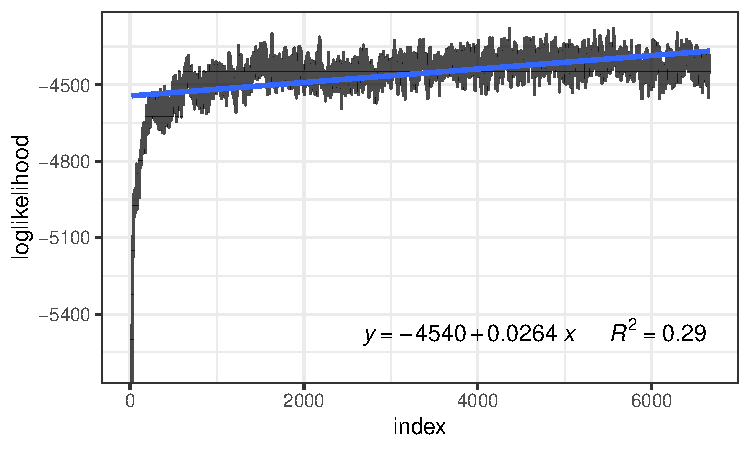
\includegraphics[scale = 0.8]{figures/mcmc_before_burnin_fitted.pdf}
	\caption{Loglikelihood values of the MCMC routine with 100,000 iterations, keeping every 15\textsuperscript{th} draw}
	\label{fig_mcmc}
\end{figure}

\begin{figure}[ht]
	\centering
  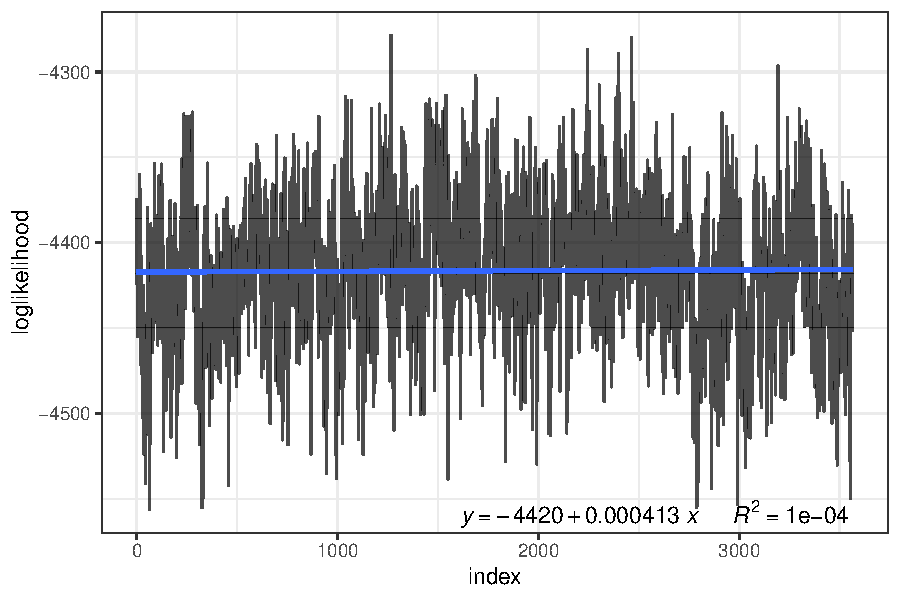
\includegraphics[scale = 0.7]{figures/mcmc_after_burnin_fitted.pdf}
	\caption{Loglikelihood values of the MCMC routine, after removing the first 3,100 observations}
	\label{fig_mcmc_burnin}
\end{figure}

The model yields the distribution of betas for all 15 brands as well as for budget and price.
Since the thorough analysis of 17 coefficients would be beyond the scope of this paper, only five presumably interesting brands\footnote{Amstel Clasica Lata, Amstel Extra Lata, Estrella Damm Lata, Estrella Galicia Lata and Heineken} were analyzed in detail.
The results for the entire data set can be found in the appendix in figures \ref{fig_corr_all} and \ref{fig_hist_all}.
A beta distribution with more probability mass in the positive domain of the density plot relative to others indicates that this brand is more preferred by the average customer.
Looking at the density plot for the beta coefficients of the five select beers (figure \ref{fig_dens_five}), there are some interesting differences in preferences:
First, Heineken has the highest mean and its distribution is visibly shifted to the right, compared to the other brands.
This indicates a higher preference for Heineken given identical prices for the average customer.
Secondly, both Estrella brands have less variant beta distributions, which hints at a less heterogeneous consumer segment.
On the other hand, both Amstel beers are characterized by high variance distributions with most probability mass in the negative domain, compared Estrella and Heineken.
That means that Amstel is the least preferred beer for many consumers in this subset and even comes with dis-utility for those customers having $\beta_{i}<0$.

\begin{figure}[ht]
	\centering
  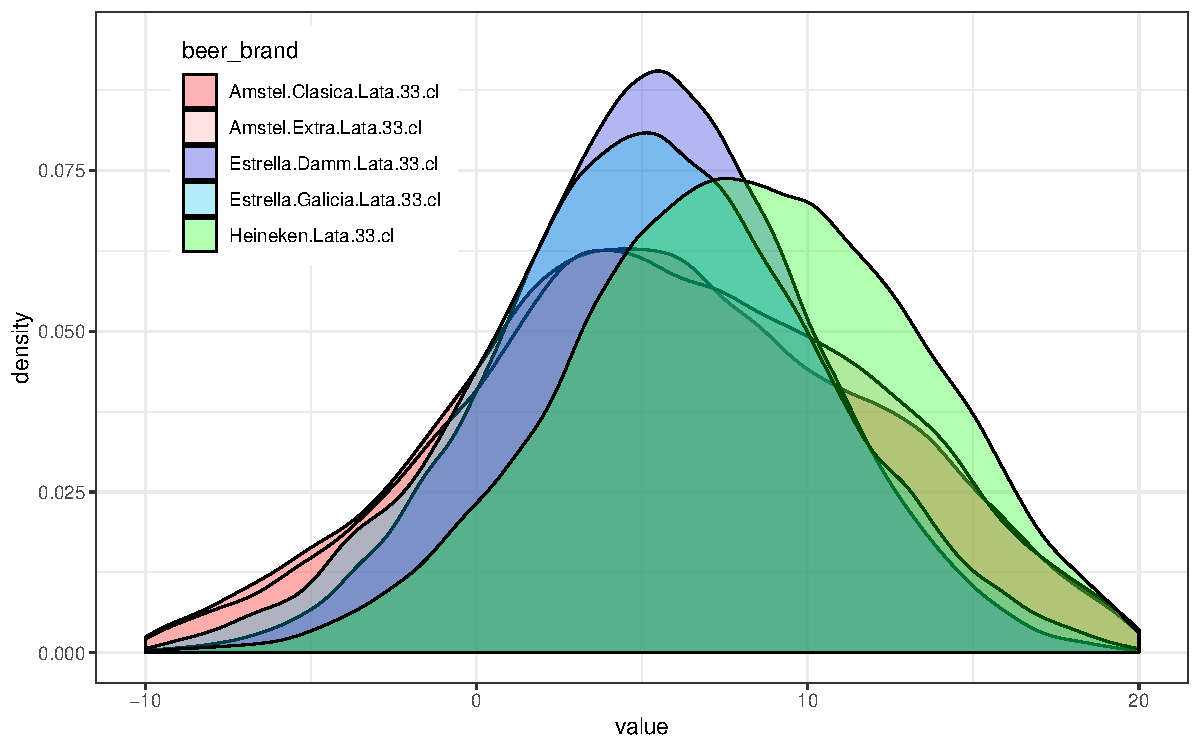
\includegraphics[scale = 0.65]{figures/dens_betas_five_in_one.pdf}
	\caption{Density plot for betas of five distinct brands}
	\label{fig_dens_five}
\end{figure}

The density plot reveals very similar preferences for both Amstel beers.
It is therefore interesting to have a look at the bivariate density plot that displays their joint beta distribution.
Figure \ref{fig_dens_amstel_biv} reveals that there is a slightly higher preference in the sample for Amstel Extra Lata compared to Amstel Clasica Lata.
This finding will subsequently explain large price discrepancies between those brands in a monopoly (see section \ref{sec_marketsim}).

\begin{figure}[ht]
	\centering
  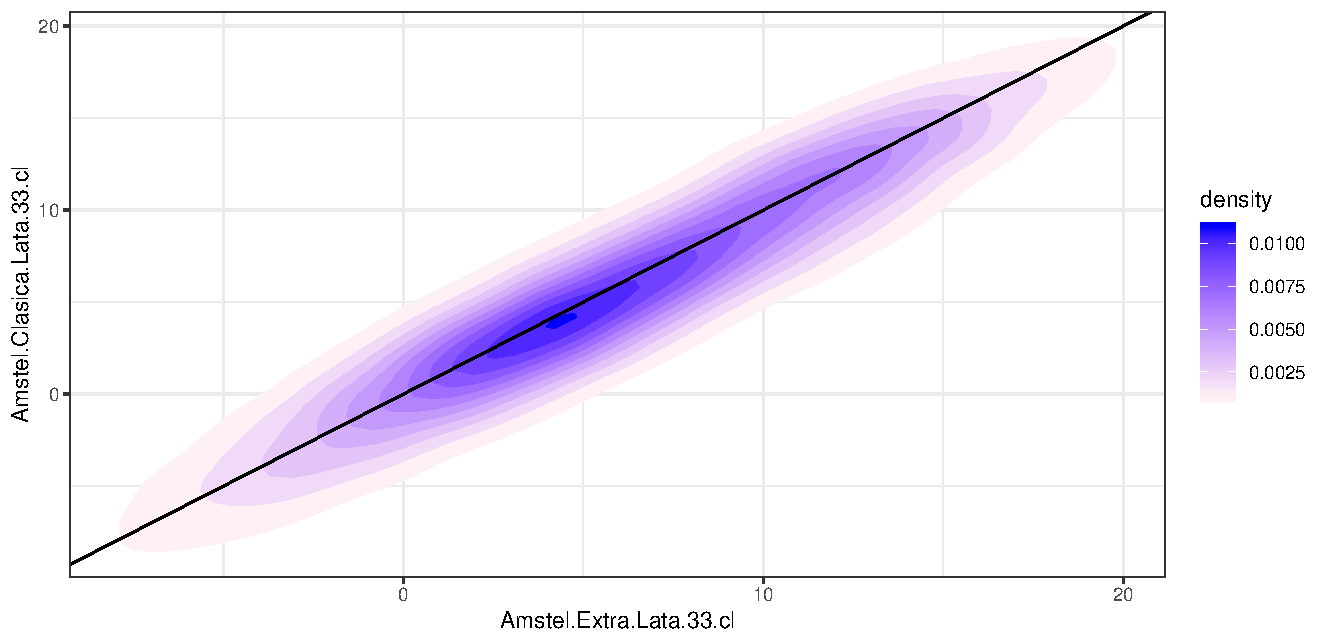
\includegraphics[scale = 0.6]{figures/amstel_bivariate_density.pdf}
	\caption{Bivariate density plot for two Amstel brands displaying slightly higher preferences for Amstel Extra Lata}
	\label{fig_dens_amstel_biv}
\end{figure}

Not only the density plots of beta distributions are of interest---their similarity in terms of correlation can quantify how similar preferences for individual brands are compared to another one.
The higher the correlation between two brands, the more similar are customers' preferences for those two beers.
Most importantly, this implicates that there is a high price-competition between those brands.
If there is a high correlation between preferences, customers regard two brands as good substitutes and therefore are mainly guided by the beer's price in their purchase decision.
Turning to the subset of beers at hand, the two Amstel brands are almost perfectly correlated ($\rho=0.95$), followed by a correlation coefficient of 0.72 and 0.75 for the Amstel brands with Heineken.
This provides a first clue that Amstel and Heineken find themselves in a strong price competition, because they serve similar customers.
Contrary to that, a low correlation between the two beta coefficients implies that those brands compete less price-wise, since they serve different segments of the market.
Especially noteworthy is that Estrella has the least correlated beta distributions compared to all other brands, which indicates that they compete least for similar customers compared to Heineken and Amstel.

Lastly, the correlation matrix also displays the correlation of betas for beer brands with betas for price.
This is an indicator how sensitive customers are to price changes.
Interestingly, customers of Estrella Galicia Lata are found to be almost completely price insensitive ($\rho=0.02$), while Heineken's customers are most influenced by price changes ($\rho=0.52$).
All else equal, a price increase by Heineken will cause a greater customer churn than the same price increase for Estrella, since the latter's customers are least price sensitive and might be influenced mainly in their purchasing decision by quality rather than price.

\begin{figure}[ht]
	\centering
  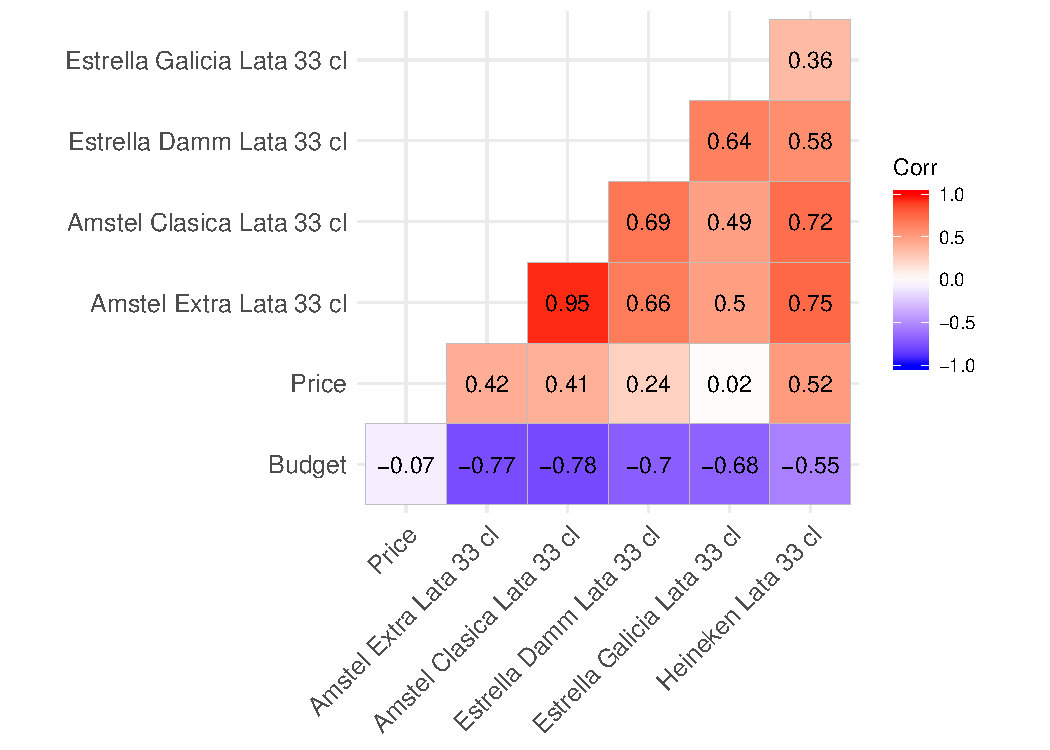
\includegraphics[scale = 0.7]{figures/corrplot_betas_five.pdf}
	\caption{Correlation of betas for price, budget and five brands}
	\label{fig_corr_five}
\end{figure}


\section{Simulating Nash Equilibria in Four Different Market Scenarios} \label{sec_marketsim}

However interesting the beta coefficients as measures of preferences might be, they do not serve as an intuitive metric and only provide a very abstract economic interpretation in terms of preferences.
To enhance the usefulness of the hierarchical Bayesian MNL model, the resulting distributions of beta coefficients can be translated into Nash equilibrium prices, shares and profits.
This section describes the beer market simulation and its results for the relevant subset of five brands in four different scenarios from full competition to monopoly.
A focus will be set on the difference between the two scenarios in the middle: brand competition and merge competition, where the first refers to a market environment before the Heineken--Amstel merger and the latter to a duopoly in which Heineken--Amstel only competes against Estrella.

To compare the different scenarios, three metrics are calculated: First, dynamic Nash equilibrium prices $p_i$, which refer to the $i^{th}$ beer's profit-optimal price.
Equilibrium price in this case means that a deviation for all players from its respective price would no longer result in a higher profit.
Based on that, the market shares $MS_i$ are computed for all brands as well as for the outside good (i.e. consumers choose to not purchase any beer).
Combining price and market share with marginal costs\footnote{as stated in section \ref{sec_vars_relat}, this study assumes constant marginal costs of $MC = 0.192 \text{ \euro}$ across all products.} enables the calculation of the product of contribution margin and market share, which is proportional to profits\footnote{no assumption about the market size is made. A simple multiplication of the market size with the formula above would yield profits.}:
\begin{align*}
Profit_i \propto (p_i - MC) * MS_i = CM_i * MS_i
\end{align*}
Those three metrics provide a clear overview over market outcomes on individual brand level.
However, it is also of high interest to quantify the aggregate market result, which can be achieved by computing the weighted average price in the market 
\begin{align*}
\bar{p}_m = \sum_{i=1}^n{p_i * MS_i},
\end{align*}
where $m$ describes the market situation and $n$ refers to the number of players plus one outside good at $p_{outside} = 0$.
By including the outside share at a price of 0, this metric quantifies a trade-off between the beers' prices and the outside share.
Higher market power leads to two changes that adversely affect $\bar{p}$: First, individual prices increase leading to an increase in $\bar{p}$.
Second, the outside share increases since some customers drop out of the market, which comes with lower inside shares and hence causes $\bar{p}$ to decrease.
If the weighted average price remained constant after a merger in the market, that means the increase in individual prices is compensated by the increase in the outside share.
This enables a conclusion about which effect dominates in certain situations.

\begin{figure}[ht]
	\centering
  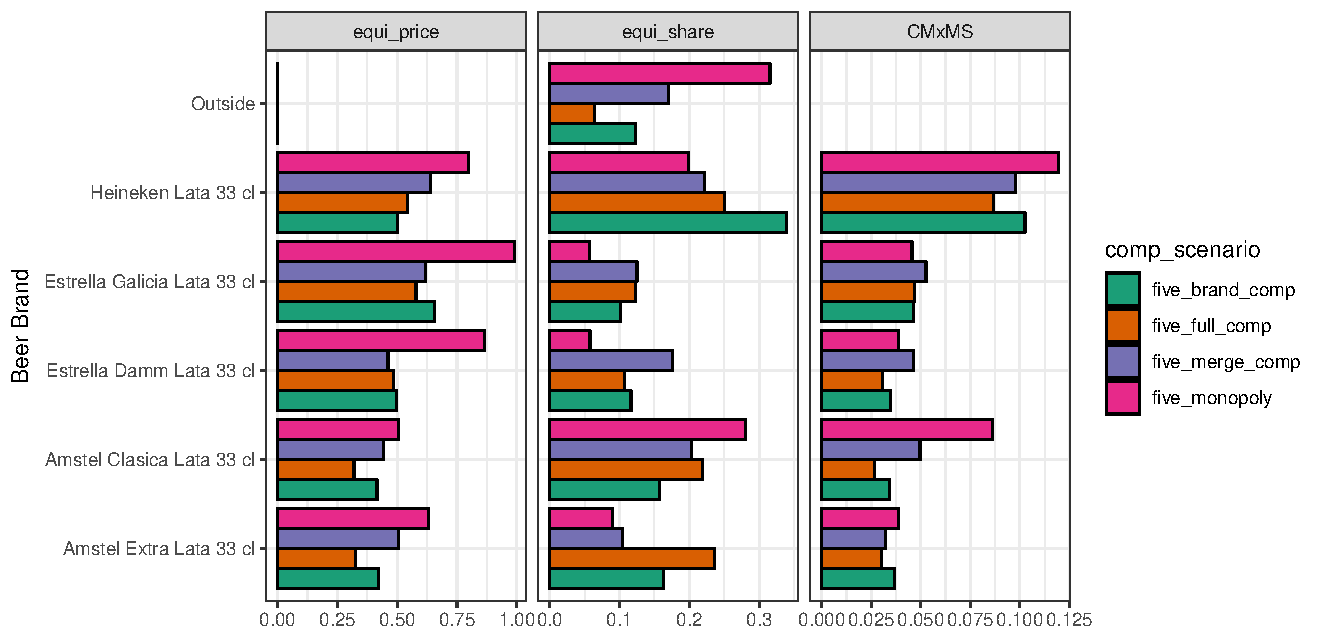
\includegraphics[scale = 0.7]{figures/bar_price_share_brand_merge_5.pdf}
	\caption{Prices and market shares in a profit-maximizing Nash equilibrium for five brands and outside option in a brand competition vs. merge setting}
	\label{fig_bar_five}
\end{figure}

Figure \ref{fig_bar_five} visualizes the market outcomes in terms of prices, market shares and profits for each of the four market scenarios.
Overall, the results appear to be in line with economic theory.
The remainder of this section discusses the individual market scenario outcomes and its implications.
Assuming full competition (i.e. all brands compete against each other), prices for most individual brands as well as $\bar{p}$ are lowest.
As expected, lowest prices come with the lowest outside share of 6.4\%.
It is interesting to note that Heineken's price is in between Amstel's (lower) and Estrella's prices (higher).
Even though it is more than 20 cents pricier than Amstel's two beers, its market share at 25\% is the highest among all beers.
This result is in line with the distribution of the model's beta coefficients.
The average consumer prefers Heineken over all other brands and Amstel is the least preferred brand.
It is therefore not surprising that even though Heineken charges higher prices than Amstel, it's market share is higher.

Now assume competition according to the beer brands, i.e. both Amstel beers, both Estrella beers, and Heineken each belong to a different owner (brand competition).
In this market of three players, weighted average prices increase from 0.41 to 0.43\text{ \euro } despite a rise in the outside share by nearly six percentage points.
A look at the individual prices suggests that thanks to its greater market power, Amstel increases their prices to nearly match Heineken's.
Remember that the correlation between the betas of Heineken and Amstel is relatively high, which means they serve similar customer segments and hence price compete strongly.
Still, Heineken's beta distribution is shifted to the right of Amstels' distributions\footnote{see figure \ref{fig_dens_amstel_biv} for the beta distribution density plots of the five beers.}, which means that consumers on average prefer Heineken over Amstel.
Since the prices of the three brands are now more similar than before, this translates to a drastic increase in Heineken's market share to more than one third of the entire market and a modest decrease in both Amstels' shares by around seven percentage points each.

The research question whether a merger between Heineken and Amstel would yield an incremental profit beyond the sum of the individual profits can now be answered by changing the ownership matrix so that those three beers belong to the same owner and thus not price compete anymore.
This market is now a duopoly with two players (Heineken together with Amstel vs. Estrella) and referred to as the merge competition scenario.
Table \ref{tab_merge} displays the weighted average price and the producer surplus before and after the merger and quantifies the absolute and relative difference between those two scenarios.
\begin{table}[!htbp] \centering 
  \caption{Weighted average prices in the entire market and producer surplus for three merged brands before vs. after the merger} 
  \label{tab_merge} 
\begin{tabular}{@{\extracolsep{10pt}} lcc}
\\[-1.8ex]\hline 
\hline \\[-1.8ex] 
 & $\bar{p}\text{ (\euro)}$ & $PS_m\text{ (\euro)}$ \\
\hline \\[-1.8ex] 
\begin{tabular}[c]{@{}l@{}}Before merger\end{tabular} & 0.428 & 0.173 \\
\begin{tabular}[c]{@{}l@{}}After merger\end{tabular} & 0.442 & 0.180 \\
$\Delta$ & +0.014 & +0.007 \\
$\Delta\%$ & +3.3\% & +3.5\% \\
\hline \\[-1.8ex] 
\end{tabular}
\end{table}
While $\bar{p}$ increases by 3.3\%, the producer surplus even increases by 3.5\%.
This represents the incremental profit due to higher market consolidation and less price competition with beer brands that targeted similar-preference customers.
The sole competitor Estrella's relative market power compared to the new Amstel--Heineken firm decreases.
Nevertheless, thanks to the consolidation, its absolute market power appears to increase.
Though their prices remain relatively constant, their profits increase due to a higher market share.
This is counter-intuitive at first---but has a logical explanation.
Looking at the distribution of beta coefficients in figure \ref{fig_dens_five}, it becomes clear that preferences are higher for Estrella than for Amstel, on average.
As Amstel's prices in this scenario approach Estrella's, the latter becomes more attractive which leads to higher market shares and profits for both Estrella beers.
In line with expectations, the outside share further increases to 17\% in the duopoly.

Based on the highest correlation of Heineken's with Amstel's preference coefficients, the incremental profit of a potential Heineken--Amstel merger was expected to be higher than a merger between brands that serve less similar consumers according to their preferences.
However, the market simulation does not support that claim.
While Heineken together with Amstel generates an additional producer surplus of 3.5\%, a merger of Heineken with the other competitor Estrella increases the sum of individual profits by 9.4\%.
The hypothesized influence of preference similarity on the incremental profits of a merger might be overruled by other market dynamics.
One possible explanation might be related to the brands' different customer segments.
While Heineken's and Estrella's prices in the brand competition scenario are similar, a merger between them would result in significantly higher prices for Estrella's brands.
This could enable a stronger customer segmentation where Estrella better captures the potential of the high-value customers, while Heineken presents itself as the preferred alternative for the medium-value customers.
Judging from the market simulation, this segmentation might be a factor that leads to a higher incremental profit of a Heineken--Estrella merger compared to a Heineken--Amstel merger, even though the latter two brands previously find themselves in higher price competition.

While the first scenario represented one extreme market constellation---full competition---the last one scrutinizes the other extreme---a monopoly.
As expected, all individual prices increase and are highest among all four scenarios.
This translates in a weighted average price of 0.46\text{ \euro }, even though almost one third of the consumers drop out of the market.
Interestingly, while all individual prices increase, the individual profits do not rise by the same magnitude due to a significant decrease in market share for most brands.
Notably, the cheapest beer in this scenario is one exception to that.
Amstel Clasica Lata at $p=0.50\text{ \euro}$ increases its profits by almost 75\% compared to the duopoly, while Amstel Extra Lata's profits only increase marginally.
This could be explained by the slightly higher preference of the average consumer for Amstel's Extra Lata beer over Clasica Lata visualized in the bivariate density plot of preferences for both brands in figure \ref{fig_dens_amstel_biv}.
Since there is no competition anymore, the firm uses this slight preference for Extra Lata and exploits the consumers' higher willingness to pay for the more preferable beer, while the remaining Amstel Clasica Lata captures all consumers that would otherwise have dropped out of the market.

This section described the outcomes in particular market scenarios and compared them to each other.
However, it is still lacking a general statement about the hypothesized relationship between price and market share (i.e. demand).
Section \ref{sec_vars_relat} stated that according to standard economic theory, a higher price should be associated with lower demand.
To check this hypothesis, figure \ref{fig_scatter_brand_comp} displays a price--market share scatterplot of all inside good market outcomes over the four market scenarios with five beer brands.

\begin{figure}[ht]
	\centering
  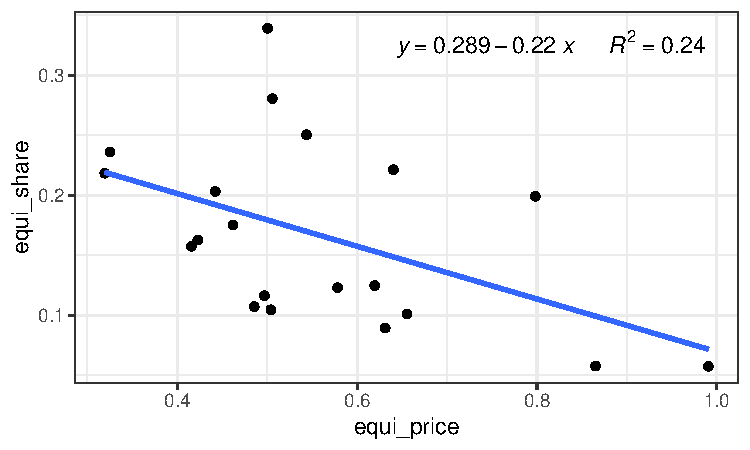
\includegraphics[scale = 0.8]{figures/scatter_price_share_all_five_scenarios.pdf}
	\caption{Price--market share scatter plot with linear regression model fit for all four competitive scenarios with five brands excluding the outside good.}
	\label{fig_scatter_brand_comp}
\end{figure}

The negative beta coefficient ($\beta_1 = -0.22$) in a simple linear regression model described by $MS_i = \beta_0 + \beta_1 * price_i + \epsilon$ suggests that this expected relationship is also reflected in the simulated market outcomes.
This is in line with the imposed constraints on the beta coefficients for price in the MNL model.
Those were assumed to be strictly positive in order to model a reward for not using up the entire budget in the BLP-type indirect utility model \citep{berryAutomobilePricesMarket1995}.
On average, an increase in beer prices of $\Delta p_i = 0.10 \text{ \euro}$, ceteris paribus is associated with a 2.2 percentage points decrease in market share. The results from this market simulation yield interesting findings for both practitioners and researchers.
Those will be discussed in the following last section.

\section{Concluding Thoughts on Managerial and Research Implications}
The implications resulting from this market simulation can be divided into two parts: The first one discusses managerial ones,
while the second part outlines suggestions for further research, especially in terms of model enhancement. 
Taking a look at the Heineken-Amstel merger from the producer's side, it generated an incremental profit of 3.5\%.
This increase in profits is solely due to higher market power and the thereby increased ability to raise prices.
Furthermore, a merger would potentially also reduce costs due to synergies, thus even increase the profits by a larger margin.
It is important to note that both players in the market benefited from the consolidation.
Even the outside party in this merger, Estrella, increased their profits compared to the scenario with three players in the market.
This indicates that in this case, Estrella's prices can be raised with less competition---even though Estrella's market power decreased relatively compared to the new Heineken--Amstel company.

With the present model and derived prices as well as market shares, it is straightforward to compute the producer surplus as the sum of individual profits.
Also, average prices considerably increase with a higher degree of market consolidation.
Consumer surplus can therefore be assumed to decrease.
Contrary to the producer surplus, the implemented methodology can however not quantify the consumer surplus for the market simulation.
When deciding whether to approve a merger of two firms from the regulator's point-of-view, economic theory argues that the overall welfare should increase \citep{perryOligopolyIncentiveHorizontal1985}.
If the producers' gains in terms of surplus outweigh the losses in consumer surplus then, strictly from an economic standpoint, the merger increases welfare and should be approved.
However, if consumers' losses were higher than producers' additional surplus, the merger would be welfare decreasing and should be prohibited.
Unfortunately, this study cannot infer any statements about this since the consumer surplus cannot be calculated with the implemented methodology.
So far, no study known to the author derives consumer welfare from a MNL model in combination with BLP-type indirect utilities.
Future research should therefore combine BLP's approach to account for budgets in MNL models with the methodology to derive consumer surplus from those models as proposed by \cite{trainWelfareCalculationsDiscrete2015}.
Weighing the losses and gains against each other would then enable well-informed decisions by regulatory authorities whether to accept or reject a merger based on welfare calculations.

\clearpage
\appendix
\section{Appendix}

\begin{figure}[ht]
	\centering
  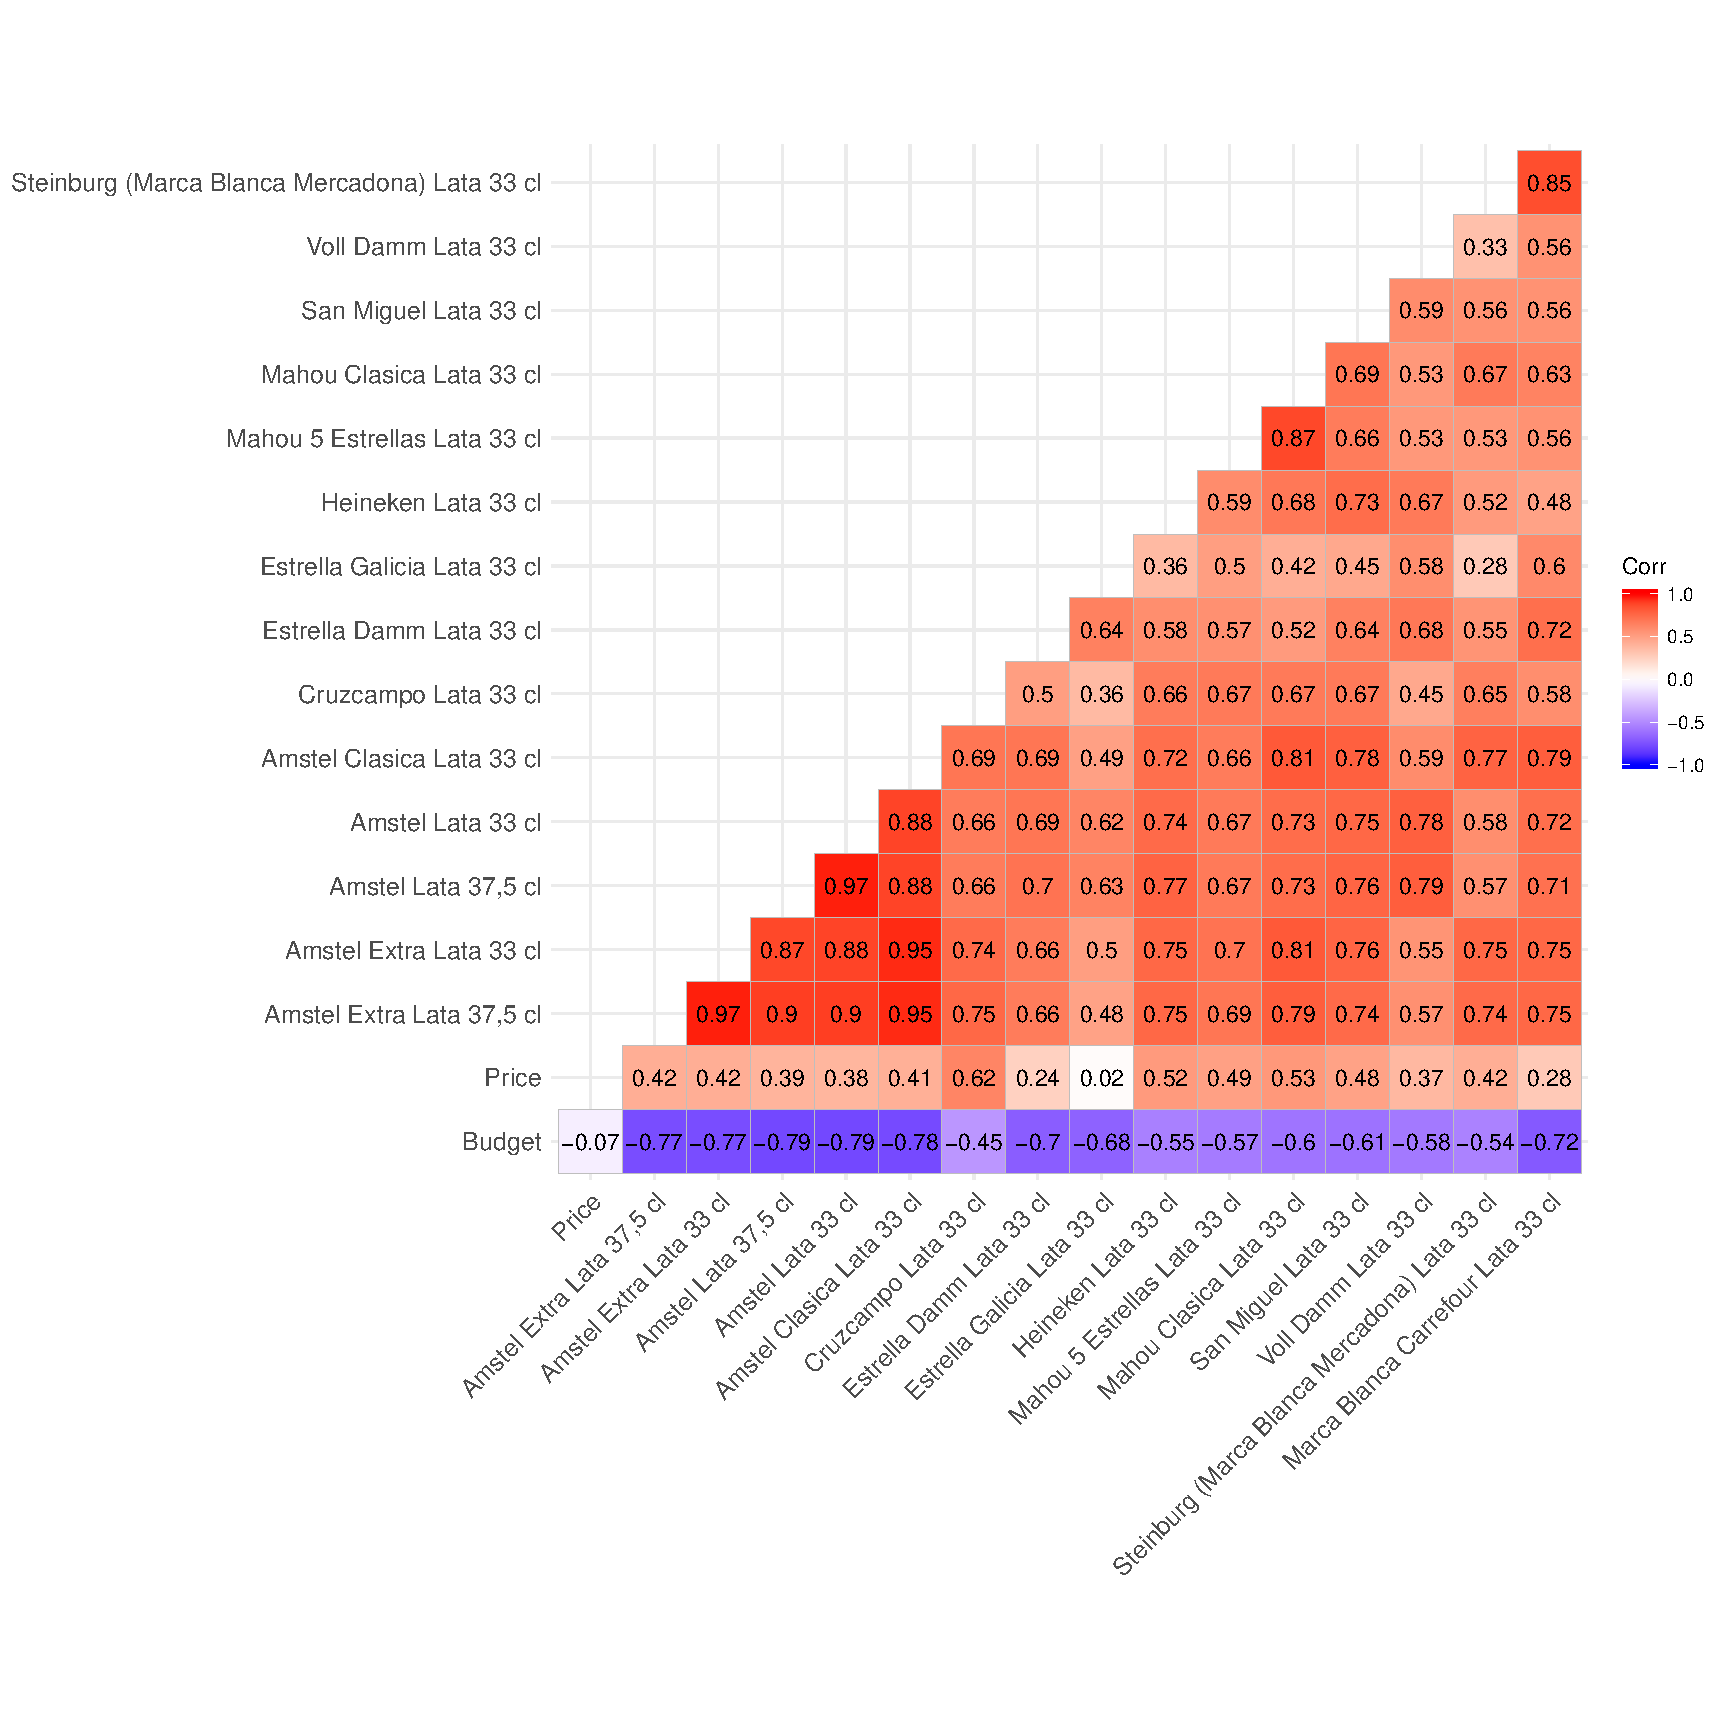
\includegraphics[scale = 0.5]{figures/corrplot_betas_full.pdf}
	\caption{Correlation of betas for price, budget and all 15 brands}
	\label{fig_corr_all}
\end{figure}

\begin{figure}[ht]
	\centering
  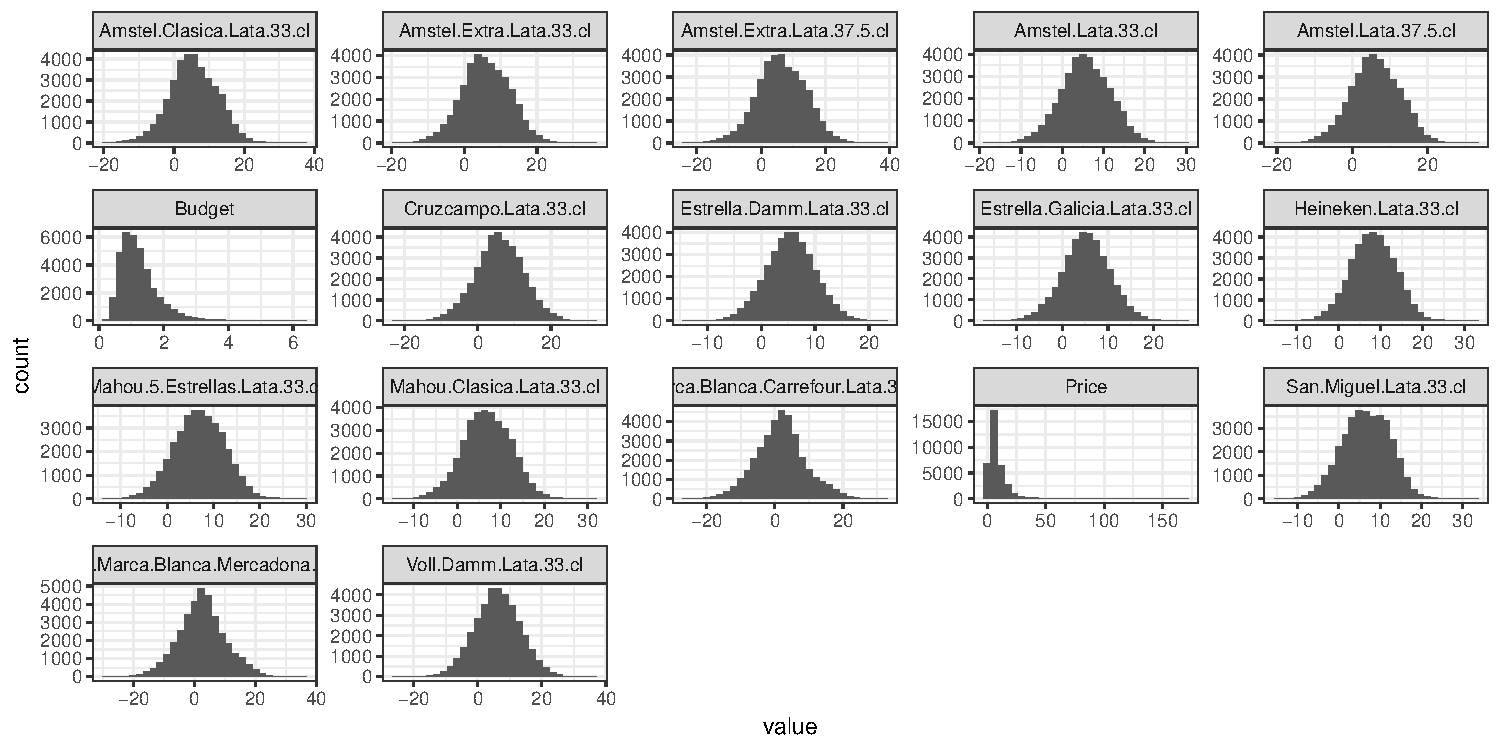
\includegraphics[scale = 0.6]{figures/hist_betas_full.pdf}
	\caption{Histograms of betas for price, budget and all 15 brands}
	\label{fig_hist_all}
\end{figure}

\begin{figure}[ht]
	\centering
  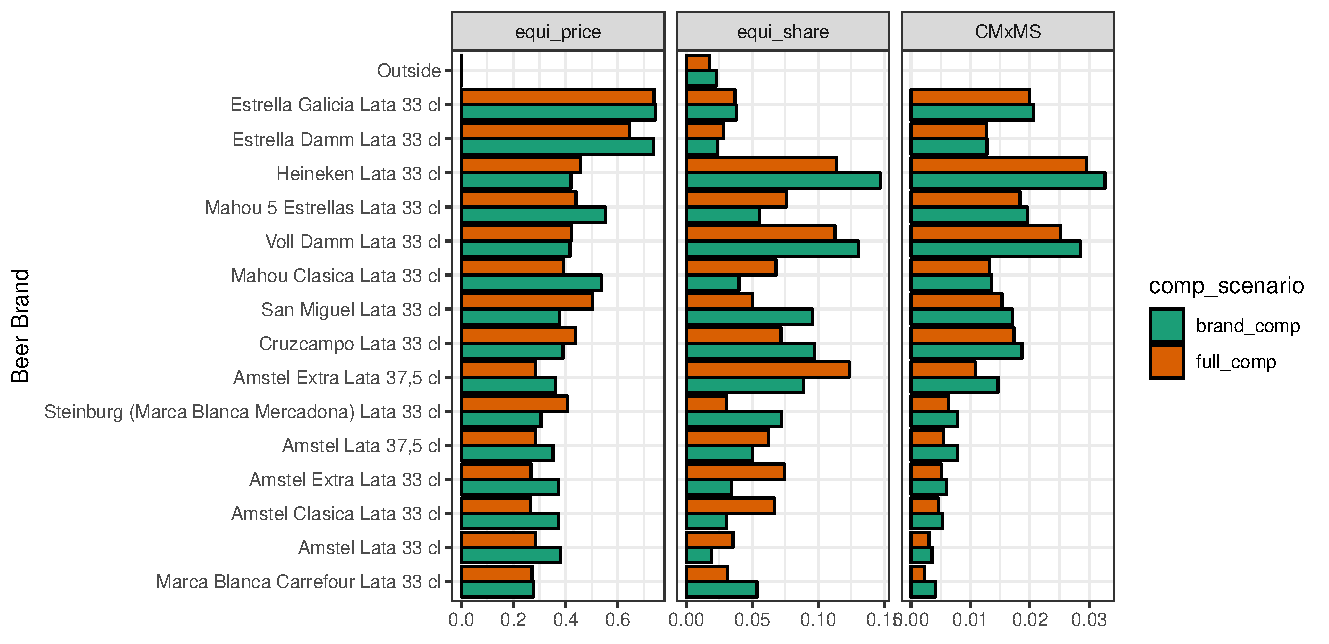
\includegraphics[scale = 0.7]{figures/bar_price_share_full_brand_15.pdf}
	\caption{Prices and market shares in a profit-maximizing Nash equilibrium for all 15 brands and outside option in a full vs. brand competition setting}
	\label{fig_bar_fifteen}
\end{figure}
\clearpage


\section{R Code}

\begin{lstlisting}[language=R,caption={Estimation of the hierarchical Bayesian MNL model and MCMC sampling routine}, label=lst_betas]
##############################################################
##### Simulation & Estimation - Nash with Budget
##### BLP-type of indirect utility
##############################################################

rm(list=ls())

# LOAD LIBRARIES
library(xtable)
library(devtools)
library(MASS)
library(Rcpp)
library(RcppArmadillo)
library(bayesm)
library(ggplot2)
library(ggpmisc)
library(tikzDevice)
library(plyr)
library(latex2exp)
library(FixedPoint)
library(dplyr)
library(reshape2)
library(tidyr)
library(ggcorrplot)

load("100k_MCMC_corrected.RData")

###Increase memory capacities
memory.limit(size=100000000)

load("Estimation_Data_Beer_20170423.Rdata")
products = c("Amstel Extra Lata 37,5 cl","Amstel Extra Lata 33 cl","Amstel Lata 37,5 cl","Amstel Lata 33 cl","Amstel Clasica Lata 33 cl",
             "Cruzcampo Lata 33 cl","Estrella Damm Lata 33 cl","Estrella Galicia Lata 33 cl","Heineken Lata 33 cl","Mahou 5 Estrellas Lata 33 cl",
             "Mahou Clasica Lata 33 cl","San Miguel Lata 33 cl","Voll Damm Lata 33 cl","Steinburg (Marca Blanca Mercadona) Lata 33 cl",
             "Marca Blanca Carrefour Lata 33 cl")

#reorder that price is first in the design matrix
for (i in 1:length(E_Data$lgtdata)){
  E_Data$lgtdata[[i]]$X <- E_Data$lgtdata[[i]]$X[,c(16,1:15)]
}

#Number of players
nplayers = 15

##########################################
#######Run BLP Budget model###############
##########################################
###Load complete sampler now...
Rcpp::sourceCpp("rhierMnlRwMixture_rcpp_loop_Illus_BLP_type.cpp",showOutput = FALSE)
source('rhierMnlRwMixture_main_untuned_BC.R')

#number of constrained coefficients (budget & price)
nvar_c = 2
#position of price coefficient in design matrix
pr=1

###Prior setting
Amu = diag(1/10, nrow = nvar_c, ncol = nvar_c)
mustarbarc = matrix(rep(0, nvar_c), nrow = nvar_c)
nu = 15 + nvar_c
V = nu * diag(nvar_c)*0.5

Prior = list(ncomp=1, Amu = Amu, mustarbarc = mustarbarc, nu = nu, V = V)
Mcmc = list(R=30000, keep=3)#, s=1.6)
#,s=c(0.1,0.5,0.5,0.5)
out_BC = rhierMnlRwMixture_SR(Data=E_Data,Prior=Prior,Mcmc=Mcmc,nvar_c=nvar_c,pr=pr,starting_budget = log(0.74))

betastar_HB_BC = out_BC$betadraw
compdraw_HB = out_BC$nmix$compdraw
probdraw_HB = out_BC$nmix$probdraw
rejection = out_BC$rejection
loglike_BC = out_BC$loglike

###Compute rejection rate of sampler 
rej_rate_indi = apply(rejection,2,mean)
summary(rej_rate_indi)
rej_rate_agg = mean(rej_rate_indi)
rej_rate_agg


########################
###Get rid of burnin####
########################

# check visually how much burn-in is required
plot(out_BC$loglike, type="l")

data.frame(loglikelihood = out_BC$loglike) %>% 
  mutate(index = row_number()) %>% 
    ggplot(aes(x = index, y = loglikelihood)) +
      geom_line(alpha = 0.7) +
      geom_smooth(method = "lm", se = FALSE) +
      stat_poly_eq(formula = y ~ x, aes(label = paste(..eq.label.., ..rr.label.., sep = "~~~~~~")), 
                   parse=TRUE,label.x.npc = "right", label.y.npc = 0.1,
                   output.type = "expression") +
  theme_bw()
      

burnin = 3100
R = dim(betastar_HB_BC)[3]

betastar_HB_BC = betastar_HB_BC[,,(burnin+1):R]
compdraw_HB = compdraw_HB[(burnin+1):R]
probdraw_HB = probdraw_HB[(burnin+1):R]
rejection = rejection[(burnin+1):R,]
loglike_BC = loglike_BC[(burnin+1):R]
plot(loglike_BC, type="l")

data.frame(loglikelihood = loglike_BC) %>% 
  mutate(index = row_number()) %>% 
  ggplot(aes(x = index, y = loglikelihood)) +
  geom_line(alpha = 0.7) +
  geom_smooth(method = "lm", se = FALSE) +
  stat_poly_eq(formula = y ~ x, aes(label = paste(..eq.label.., ..rr.label.., sep = "~~~~~~")), 
               parse=TRUE,label.x.npc = "right", label.y.npc = 0.01,
               output.type = "expression") +
  theme_bw()


lmdata <- data.frame(loglikelihood = loglike_BC) %>% 
  mutate(index = row_number())
lm(loglike_BC ~ index, data = lmdata) %>% 
          summary()

R = dim(betastar_HB_BC)[3]
N = dim(betastar_HB_BC)[1]

###Heterogeneity distribution lower level model non-smoothed  
l=10
betastar_BC_LLMns <- array(0,dim=c(R*l,dim(betastar_HB_BC)[2]))
index_r = rep(rank(runif(R)),l)
index_n = rep(rank(runif(N)),round((R*l)/N)+1)

#data generation
for(i in 1:(R*l)){
  betastar_BC_LLMns[i,] = betastar_HB_BC[index_n[i],,index_r[i]]
}
#transform betastardraws to betadraws
beta_BC_LLMns = betastar_BC_LLMns
beta_BC_LLMns[,1] = exp(betastar_BC_LLMns[,1])
beta_BC_LLMns[,2] = exp(betastar_BC_LLMns[,2])

summary(beta_BC_LLMns)
\end{lstlisting}
\begin{lstlisting}[language=R,caption={Computing dynamic Nash equilibria in different competitive scenarios via the fixed point algorithm}, label=lst_nash_esti]
#######################  
###Nash optimization
#######################

### Load functions for Fixed-point approach
source('Morrow_Skerlos_Implementations_BC_BLP_MarkupEquations_Final_Efficient.R')
Rcpp::sourceCpp("Speed++_MS_BC_BLP_Efficient.cpp",showOutput = FALSE)

###########################################################################
# Nash Equilibrium Prices and Shares for all 15 brands
###########################################################################

# ingredients
nplayers = 15 + 1 ### 15 inside + outside
min_p = 0.22
prices_init = c(rep(min_p,nplayers - 1),0)
designBase = rbind(diag(nplayers-1),rep(0,nplayers-1))
Xdata = cbind(prices_init,designBase); colnames(Xdata)[1] = "PRICE" 
Ownership = array(0,dim=c(nplayers,nplayers))
Ownership[1:(nplayers-1),1:(nplayers-1)] = diag((nplayers-1))

# define which brands compete on price, i.e. are owned by different companies
# without any specification, all brands compete (owned by different companies)
#Ownership[1,2] <- 1
#Ownership[2,1] <- 1

inside_row=which(rowSums(Ownership) != 0, arr.ind = TRUE)
p0=Xdata[inside_row,"PRICE"]
costBase = as.vector(prices_init*0.9)
MC = costBase[inside_row]

### Run Fixed-Point algorithm with Xi-markup equation (reliable and fast: See Table 3 in paper for comparison)
p_Markup_Xi_FixedPoint_BC_BLP = FixedPoint(Function = function(price_vec) FixedPoint_BLP_Xi(price_vec,MC=MC, ownership=Ownership,Xdata=Xdata,beta_draws=beta_BC_LLMns,pr=1), Inputs = p0, MaxIter = 10000, ConvergenceMetricThreshold = 1e-10, Method = "Anderson")

p_Markup_Xi_FixedPoint_BC_BLP$FixedPoint

# Overview optimal prices & shares
Optimal_prices <- array(0,dim=c(nplayers,2))
rownames(Optimal_prices) = c(products[1:(nplayers-1)],"Outside")
colnames(Optimal_prices) = c("Equilibrium Price","Equilibrium Shares")
# Save equi-prices
Optimal_prices[,"Equilibrium Price"] <-c(p_Markup_Xi_FixedPoint_BC_BLP$FixedPoint,0)
# Check for all of the 15 brands -> change one, keep all the others fixed
computeShares_BC_BLP <- function(prices, beta, design, pr = 1) {
  fullDesign <- cbind(prices,design) ###put prices to the last position here
  probabilities_BC_BLP_log_cpp(beta,fullDesign,pr)
}
Optimal_prices[,"Equilibrium Shares"] <- as.vector(computeShares_BC_BLP(Optimal_prices[,"Equilibrium Price"], beta_BC_LLMns,designBase,pr=1))
round(Optimal_prices,2)

# store results in data frame
res_matrix <- data.frame(
  product = c(products[1:(nplayers-1)],"Outside"),
  equi_price = as.numeric(c(p_Markup_Xi_FixedPoint_BC_BLP$FixedPoint,0)),
  equi_share = as.vector(computeShares_BC_BLP(Optimal_prices[,"Equilibrium Price"],
                                              beta_BC_LLMns,designBase,pr=1)))

# create list to store different competitive scenarios
scenarios <- list("full_comp" = res_matrix)

###########################################################################
# Ownership according to brand names (ie all Amstel go to the same company)
###########################################################################

# ingredients
nplayers = 15 + 1 ### 15 inside + outside
min_p = 0.22
prices_init = c(rep(min_p,nplayers - 1),0)
designBase = rbind(diag(nplayers-1),rep(0,nplayers-1))
Xdata = cbind(prices_init,designBase); colnames(Xdata)[1] = "PRICE" 
Ownership = array(0,dim=c(nplayers,nplayers))
Ownership[1:(nplayers-1),1:(nplayers-1)] = diag((nplayers-1))

# define which brands compete on price, i.e. are owned by different companies
# Amstel (five brands)
for (i in 1:5){
  for (k in 1:5){
    Ownership[i,k] <- 1
  }
}
# Estrella (two brands)
for (i in 7:8){
  for (k in 7:8){
    Ownership[i,k] <- 1
  }
}
# Mahou (two brands)
for (i in 10:11){
  for (k in 10:11){
    Ownership[i,k] <- 1
  }
}

inside_row=which(rowSums(Ownership) != 0, arr.ind = TRUE)
p0=Xdata[inside_row,"PRICE"]
costBase = as.vector(prices_init*0.9)
MC = costBase[inside_row]

### Run Fixed-Point algorithm with Xi-markup equation (reliable and fast: See Table 3 in paper for comparison)
p_Markup_Xi_FixedPoint_BC_BLP = FixedPoint(Function = function(price_vec) FixedPoint_BLP_Xi(price_vec,MC=MC, ownership=Ownership,Xdata=Xdata,beta_draws=beta_BC_LLMns,pr=1),  Inputs = p0, MaxIter = 10000, ConvergenceMetricThreshold = 1e-10, Method = "Anderson")

p_Markup_Xi_FixedPoint_BC_BLP$FixedPoint

Optimal_prices <- array(0,dim=c(nplayers,2))
rownames(Optimal_prices) = c(products[1:(nplayers-1)],"Outside")
colnames(Optimal_prices) = c("Equilibrium Price","Equilibrium Shares")
# Save equi-prices
Optimal_prices[,"Equilibrium Price"] <-c(p_Markup_Xi_FixedPoint_BC_BLP$FixedPoint,0)
computeShares_BC_BLP <- function(prices, beta, design, pr = 1) {
  fullDesign <- cbind(prices,design) ###put prices to the last position here
  probabilities_BC_BLP_log_cpp(beta,fullDesign,pr)
}
Optimal_prices[,"Equilibrium Shares"] <- as.vector(computeShares_BC_BLP(Optimal_prices[,"Equilibrium Price"], beta_BC_LLMns,designBase,pr=1))

round(Optimal_prices,2)

# store results in data frame
res_matrix <- data.frame(
  product = c(products[1:(nplayers-1)],"Outside"),
  equi_price = as.numeric(c(p_Markup_Xi_FixedPoint_BC_BLP$FixedPoint,0)),
  equi_share = as.vector(computeShares_BC_BLP(Optimal_prices[,"Equilibrium Price"],
                                       beta_BC_LLMns,designBase,pr=1)))


# add to results list
scenarios[["brand_comp"]] <- res_matrix


###########################################################################
# Only two Amstel, two Estrella and one Heineken (Ownership according to brands)
###########################################################################

# ingredients
nplayers = 5 + 1 
min_p = 0.22
prices_init = c(rep(min_p,nplayers - 1),0)
designBase = rbind(diag(nplayers-1),rep(0,nplayers-1))
Xdata = cbind(prices_init,designBase); colnames(Xdata)[1] = "PRICE" 
Ownership = array(0,dim=c(nplayers,nplayers))
Ownership[1:(nplayers-1),1:(nplayers-1)] = diag((nplayers-1))

# define which brands compete on price, i.e. are owned by different companies
# Amstel (two brands)
for (i in 1:2){
  for (k in 1:2){
    Ownership[i,k] <- 1
  }
}
# Estrella (two brands)
for (i in 3:4){
  for (k in 3:4){
    Ownership[i,k] <- 1
  }
}


inside_row=which(rowSums(Ownership) != 0, arr.ind = TRUE)
p0=Xdata[inside_row,"PRICE"]
costBase = as.vector(prices_init*0.9)
MC = costBase[inside_row]

### Run Fixed-Point algorithm with Xi-markup equation (reliable and fast: See Table 3 in paper for comparison)
p_Markup_Xi_FixedPoint_BC_BLP = FixedPoint(Function = function(price_vec) FixedPoint_BLP_Xi(price_vec,MC=MC, ownership=Ownership,Xdata=Xdata,beta_draws=beta_BC_LLMns[,(c(1,2,4,7,9,10,11))],pr=1), Inputs = p0, MaxIter = 10000, ConvergenceMetricThreshold = 1e-10, Method = "Anderson")

p_Markup_Xi_FixedPoint_BC_BLP$FixedPoint

Optimal_prices <- array(0,dim=c(nplayers,2))
rownames(Optimal_prices) = c(products[c(2,5,7,8,9)],"Outside")
colnames(Optimal_prices) = c("Equilibrium Price","Equilibrium Shares")
# Save equi-prices
Optimal_prices[,"Equilibrium Price"] <-c(p_Markup_Xi_FixedPoint_BC_BLP$FixedPoint,0)
computeShares_BC_BLP <- function(prices, beta, design, pr = 1) {
  fullDesign <- cbind(prices,design) ###put prices to the last position here
  probabilities_BC_BLP_log_cpp(beta,fullDesign,pr)
}
Optimal_prices[,"Equilibrium Shares"] <- as.vector(computeShares_BC_BLP(Optimal_prices[,"Equilibrium Price"], beta_BC_LLMns[,c(1,2,4,7,9,10,11)],designBase,pr=1))

round(Optimal_prices,2)

# store results in data frame
res_matrix <- data.frame(
  product = rownames(Optimal_prices),
  equi_price = as.numeric(c(p_Markup_Xi_FixedPoint_BC_BLP$FixedPoint,0)),
  equi_share = as.vector(computeShares_BC_BLP(Optimal_prices[,"Equilibrium Price"],
                                              beta_BC_LLMns[,c(1,2,4,7,9,10,11)],designBase,pr=1)))


# add to results list
scenarios[["five_full_comp"]] <- res_matrix

###########################################################################
# Only two Amstel, two Estrella and one Heineken (Merger Amstel and Heineken, bc highly correlated betas)
###########################################################################

# ingredients
nplayers = 5 + 1 
min_p = 0.22
prices_init = c(rep(min_p,nplayers - 1),0)
designBase = rbind(diag(nplayers-1),rep(0,nplayers-1))
Xdata = cbind(prices_init,designBase); colnames(Xdata)[1] = "PRICE" 
Ownership = array(0,dim=c(nplayers,nplayers))
Ownership[1:(nplayers-1),1:(nplayers-1)] = diag((nplayers-1))

# define which brands compete on price, i.e. are owned by different companies
# Amstel (two brands)
for (i in c(1:2,5)){
  for (k in c(1:2,5)){
    Ownership[i,k] <- 1
  }
}
# Estrella (two brands)
for (i in 3:4){
  for (k in 3:4){
    Ownership[i,k] <- 1
  }
}

inside_row=which(rowSums(Ownership) != 0, arr.ind = TRUE)
p0=Xdata[inside_row,"PRICE"]
costBase = as.vector(prices_init*0.9)
MC = costBase[inside_row]

### Run Fixed-Point algorithm with Xi-markup equation (reliable and fast: See Table 3 in paper for comparison)
p_Markup_Xi_FixedPoint_BC_BLP = FixedPoint(Function = function(price_vec) FixedPoint_BLP_Xi(price_vec,MC=MC, ownership=Ownership,Xdata=Xdata,beta_draws=beta_BC_LLMns[,(c(1,2,4,7,9,10,11))],pr=1), Inputs = p0, MaxIter = 10000, ConvergenceMetricThreshold = 1e-10, Method = "Anderson")

p_Markup_Xi_FixedPoint_BC_BLP$FixedPoint

Optimal_prices <- array(0,dim=c(nplayers,2))
rownames(Optimal_prices) = c(products[c(2,5,7,8,9)],"Outside")
colnames(Optimal_prices) = c("Equilibrium Price","Equilibrium Shares")
# Save equi-prices
Optimal_prices[,"Equilibrium Price"] <-c(p_Markup_Xi_FixedPoint_BC_BLP$FixedPoint,0)
computeShares_BC_BLP <- function(prices, beta, design, pr = 1) {
  fullDesign <- cbind(prices,design) ###put prices to the last position here
  probabilities_BC_BLP_log_cpp(beta,fullDesign,pr)
}
Optimal_prices[,"Equilibrium Shares"] <- as.vector(computeShares_BC_BLP(Optimal_prices[,"Equilibrium Price"], beta_BC_LLMns[,c(1,2,4,7,9,10,11)],designBase,pr=1))

round(Optimal_prices,2)

# store results in data frame
res_matrix <- data.frame(
  product = rownames(Optimal_prices),
  equi_price = as.numeric(c(p_Markup_Xi_FixedPoint_BC_BLP$FixedPoint,0)),
  equi_share = as.vector(computeShares_BC_BLP(Optimal_prices[,"Equilibrium Price"],
                                              beta_BC_LLMns[,c(1,2,4,7,9,10,11)],designBase,pr=1)))


# add to results list
scenarios[["five_merge_comp"]] <- res_matrix

###########################################################################
# Heineken and Estrella Merger
###########################################################################

# ingredients
nplayers = 5 + 1 
min_p = 0.22
prices_init = c(rep(min_p,nplayers - 1),0)
designBase = rbind(diag(nplayers-1),rep(0,nplayers-1))
Xdata = cbind(prices_init,designBase); colnames(Xdata)[1] = "PRICE" 
Ownership = array(0,dim=c(nplayers,nplayers))
Ownership[1:(nplayers-1),1:(nplayers-1)] = diag((nplayers-1))

# define which brands compete on price, i.e. are owned by different companies
# Amstel (two brands)
for (i in c(1:2)){
  for (k in c(1:2)){
    Ownership[i,k] <- 1
  }
}
# Estrella (two brands)
for (i in c(3:4,5)){
  for (k in c(3:4,5)){
    Ownership[i,k] <- 1
  }
}

inside_row=which(rowSums(Ownership) != 0, arr.ind = TRUE)
p0=Xdata[inside_row,"PRICE"]
costBase = as.vector(prices_init*0.9)
MC = costBase[inside_row]

### Run Fixed-Point algorithm with Xi-markup equation (reliable and fast: See Table 3 in paper for comparison)
p_Markup_Xi_FixedPoint_BC_BLP = FixedPoint(Function = function(price_vec) FixedPoint_BLP_Xi(price_vec,MC=MC, ownership=Ownership,Xdata=Xdata,beta_draws=beta_BC_LLMns[,(c(1,2,4,7,9,10,11))],pr=1), Inputs = p0, MaxIter = 10000, ConvergenceMetricThreshold = 1e-10, Method = "Anderson")

p_Markup_Xi_FixedPoint_BC_BLP$FixedPoint

Optimal_prices <- array(0,dim=c(nplayers,2))
rownames(Optimal_prices) = c(products[c(2,5,7,8,9)],"Outside")
colnames(Optimal_prices) = c("Equilibrium Price","Equilibrium Shares")
# Save equi-prices
Optimal_prices[,"Equilibrium Price"] <-c(p_Markup_Xi_FixedPoint_BC_BLP$FixedPoint,0)
computeShares_BC_BLP <- function(prices, beta, design, pr = 1) {
  fullDesign <- cbind(prices,design) ###put prices to the last position here
  probabilities_BC_BLP_log_cpp(beta,fullDesign,pr)
}
Optimal_prices[,"Equilibrium Shares"] <- as.vector(computeShares_BC_BLP(Optimal_prices[,"Equilibrium Price"], beta_BC_LLMns[,c(1,2,4,7,9,10,11)],designBase,pr=1))

round(Optimal_prices,2)

# store results in data frame
res_matrix <- data.frame(
  product = rownames(Optimal_prices),
  equi_price = as.numeric(c(p_Markup_Xi_FixedPoint_BC_BLP$FixedPoint,0)),
  equi_share = as.vector(computeShares_BC_BLP(Optimal_prices[,"Equilibrium Price"],
                                              beta_BC_LLMns[,c(1,2,4,7,9,10,11)],designBase,pr=1)))


# add to results list
scenarios[["five_merge_comp_estr"]] <- res_matrix

###########################################################################
# Only two Amstel, two Estrella and one Heineken (Full Competition)
###########################################################################

# ingredients
nplayers = 5 + 1 
min_p = 0.22
prices_init = c(rep(min_p,nplayers - 1),0)
designBase = rbind(diag(nplayers-1),rep(0,nplayers-1))
Xdata = cbind(prices_init,designBase); colnames(Xdata)[1] = "PRICE" 
Ownership = array(0,dim=c(nplayers,nplayers))
Ownership[1:(nplayers-1),1:(nplayers-1)] = diag((nplayers-1))

inside_row=which(rowSums(Ownership) != 0, arr.ind = TRUE)
p0=Xdata[inside_row,"PRICE"]
costBase = as.vector(prices_init*0.9)
MC = costBase[inside_row]

### Run Fixed-Point algorithm with Xi-markup equation (reliable and fast: See Table 3 in paper for comparison)
p_Markup_Xi_FixedPoint_BC_BLP = FixedPoint(Function = function(price_vec) FixedPoint_BLP_Xi(price_vec,MC=MC, ownership=Ownership,Xdata=Xdata,beta_draws=beta_BC_LLMns[,(c(1,2,4,7,9,10,11))],pr=1),  Inputs = p0, MaxIter = 10000, ConvergenceMetricThreshold = 1e-10, Method = "Anderson")

p_Markup_Xi_FixedPoint_BC_BLP$FixedPoint

Optimal_prices <- array(0,dim=c(nplayers,2))
rownames(Optimal_prices) = c(products[c(2,5,7,8,9)],"Outside")
colnames(Optimal_prices) = c("Equilibrium Price","Equilibrium Shares")
# Save equi-prices
Optimal_prices[,"Equilibrium Price"] <-c(p_Markup_Xi_FixedPoint_BC_BLP$FixedPoint,0)
computeShares_BC_BLP <- function(prices, beta, design, pr = 1) {
  fullDesign <- cbind(prices,design) ###put prices to the last position here
  probabilities_BC_BLP_log_cpp(beta,fullDesign,pr)
}
Optimal_prices[,"Equilibrium Shares"] <- as.vector(computeShares_BC_BLP(Optimal_prices[,"Equilibrium Price"], beta_BC_LLMns[,c(1,2,4,7,9,10,11)],designBase,pr=1))

round(Optimal_prices,2)

# store results in data frame
res_matrix <- data.frame(
  product = rownames(Optimal_prices),
  equi_price = as.numeric(c(p_Markup_Xi_FixedPoint_BC_BLP$FixedPoint,0)),
  equi_share = as.vector(computeShares_BC_BLP(Optimal_prices[,"Equilibrium Price"],
                                              beta_BC_LLMns[,c(1,2,4,7,9,10,11)],designBase,pr=1)))


# add to results list
scenarios[["five_full_comp"]] <- res_matrix

###########################################################################
# Only two Amstel, two Estrella and one Heineken (Monopoly)
###########################################################################

# ingredients
nplayers = 5 + 1 
min_p = 0.22
prices_init = c(rep(min_p,nplayers - 1),0)
designBase = rbind(diag(nplayers-1),rep(0,nplayers-1))
Xdata = cbind(prices_init,designBase); colnames(Xdata)[1] = "PRICE" 
Ownership = array(0,dim=c(nplayers,nplayers))
Ownership[1:(nplayers-1),1:(nplayers-1)] = diag((nplayers-1))

# define which brands compete on price, i.e. are owned by different companies
# All five belong to the same owner
for (i in 1:5){
  for (k in 1:5){
    Ownership[i,k] <- 1
  }
}

inside_row=which(rowSums(Ownership) != 0, arr.ind = TRUE)
p0=Xdata[inside_row,"PRICE"]
costBase = as.vector(prices_init*0.9)
MC = costBase[inside_row]

### Run Fixed-Point algorithm with Xi-markup equation (reliable and fast: See Table 3 in paper for comparison)
p_Markup_Xi_FixedPoint_BC_BLP = FixedPoint(Function = function(price_vec) FixedPoint_BLP_Xi(price_vec,MC=MC, ownership=Ownership,Xdata=Xdata,beta_draws=beta_BC_LLMns[,(c(1,2,4,7,9,10,11))],pr=1),  Inputs = p0, MaxIter = 10000, ConvergenceMetricThreshold = 1e-10, Method = "Anderson")

p_Markup_Xi_FixedPoint_BC_BLP$FixedPoint

Optimal_prices <- array(0,dim=c(nplayers,2))
rownames(Optimal_prices) = c(products[c(2,5,7,8,9)],"Outside")
colnames(Optimal_prices) = c("Equilibrium Price","Equilibrium Shares")
# Save equi-prices
Optimal_prices[,"Equilibrium Price"] <-c(p_Markup_Xi_FixedPoint_BC_BLP$FixedPoint,0)
computeShares_BC_BLP <- function(prices, beta, design, pr = 1) {
  fullDesign <- cbind(prices,design) ###put prices to the last position here
  probabilities_BC_BLP_log_cpp(beta,fullDesign,pr)
}
Optimal_prices[,"Equilibrium Shares"] <- as.vector(computeShares_BC_BLP(Optimal_prices[,"Equilibrium Price"], beta_BC_LLMns[,c(1,2,4,7,9,10,11)],designBase,pr=1))

round(Optimal_prices,2)

# store results in data frame
res_matrix <- data.frame(
  product = rownames(Optimal_prices),
  equi_price = as.numeric(c(p_Markup_Xi_FixedPoint_BC_BLP$FixedPoint,0)),
  equi_share = as.vector(computeShares_BC_BLP(Optimal_prices[,"Equilibrium Price"],
                                              beta_BC_LLMns[,c(1,2,4,7,9,10,11)],designBase,pr=1)))


# add to results list
scenarios[["five_monopoly"]] <- res_matrix
\end{lstlisting}
\begin{lstlisting}[language=R,caption={Computation of weighed average prices and profits (i.e. $CMxMS$)}, label=lst_compute_metrics]
########################################################
# Compute Average Prices in the Market, Weighted by Market Share
########################################################

w_a_p_full_comp <- t(scenarios[["full_comp"]]$equi_price) %*% scenarios[["full_comp"]]$equi_share
w_a_p_brand_comp <- t(scenarios[["brand_comp"]]$equi_price) %*% scenarios[["brand_comp"]]$equi_share

w_a_p_five_full_comp <- t(scenarios[["five_full_comp"]]$equi_price) %*% scenarios[["five_full_comp"]]$equi_share
w_a_p_five_brand_comp <- t(scenarios[["five_brand_comp"]]$equi_price) %*% scenarios[["five_brand_comp"]]$equi_share
w_a_p_five_monopoly <- t(scenarios[["five_monopoly"]]$equi_price) %*% scenarios[["five_monopoly"]]$equi_share
w_a_p_five_merge <- t(scenarios[["five_merge_comp"]]$equi_price) %*% scenarios[["five_merge_comp"]]$equi_share
w_a_p_five_merge_estr <- t(scenarios[["five_merge_comp_estr"]]$equi_price) %*% scenarios[["five_merge_comp_estr"]]$equi_share

w_a_p_brand_comp / w_a_p_full_comp
w_a_p_five_brand_comp / w_a_p_five_full_comp

# compute average annual welfare loss for typical German consumer with the merger
welf_loss_avg <- 102/(1/3)*(w_a_p_five_merge - w_a_p_five_brand_comp)
welf_loss_total <- welf_loss_avg * 82000000


########################################################
# Compute contribution margin * market share for all scenarios
########################################################
MC <- rep(0.198, 15)
for (i in 1:length(scenarios)) { #
  # position of outside good
  out_pos <- length(scenarios[[i]]$equi_price)
  
  # compute contribubtion margin times market share for every brand in every scenario in the list
  scenarios[[i]]$CMxMS <- c((scenarios[[i]][-out_pos,"equi_price"] - MC[1:out_pos-1]) * scenarios[[i]][-out_pos,"equi_share"], NA)
  
}

# compute CMxMS for both Amstel and Heineken before and after merger
CMxMS_full_comp <- sum(scenarios$five_full_comp[c(1,2,5),"CMxMS"])
CMxMS_before <- sum(scenarios$five_brand_comp[c(1,2,5),"CMxMS"])
CMxMS_after <- sum(scenarios$five_merge_comp[c(1,2,5),"CMxMS"])
CMxMS_monop <- sum(scenarios$five_monopoly[c(1,2,5),"CMxMS"])

CMxMS_before_estr <- sum(scenarios$five_brand_comp[c(3:5),"CMxMS"])
CMxMS_after_estr <- sum(scenarios$five_merge_comp_estr[c(3:5),"CMxMS"])


CMxMS_after / CMxMS_before
CMxMS_monop / CMxMS_full_comp
CMxMS_monop / CMxMS_after

CMxMS_after_estr / CMxMS_before_estr

\end{lstlisting}
\begin{lstlisting}[language=R,caption={Plotting correlations, beta densities, histograms, market outcomes, and a price-market share scatterplot}, label=lst_plotting]
########################################################
# Plotting
########################################################

# corrplot of betas for all 15 brands
colnames(beta_BC_LLMns) <- c("Budget", "Price", products)
windows()
cor(beta_BC_LLMns) %>% 
  ggcorrplot(type = "lower", lab = TRUE)

cor(beta_BC_LLMns[,c(1,2,4,7,9,10,11)]) %>% 
  ggcorrplot(type = "lower", lab = TRUE)


# histogram of all betas
beta_BC_LLMns %>% 
    data.frame() %>% 
      gather(key = "beer_brand") %>% 
        ggplot(aes(value)) +
          geom_histogram() +
          facet_wrap(~beer_brand, scales = "free") +
          theme_bw()

# density plot of five brands (all in one)
beta_BC_LLMns[,c(4,7,9,10,11)] %>% 
  data.frame() %>% 
  gather(key = "beer_brand") %>% 
  ggplot(aes(value)) +
  geom_density(aes(fill = beer_brand), position="identity", alpha = 0.3) +
  xlim(c(-10, 20)) +
  ylim(c(0, 0.095)) +
  scale_fill_manual(values = c("#FD0505", "#FF9A9A", "#000CD3", "#00C1EA", "green")) +
  theme_bw() +
  theme(legend.position = c(0.2, 0.8),
        legend.direction = "vertical")

# density plot of five brands (separate)
beta_BC_LLMns[,c(2,4,7,9,10,11)] %>% 
  data.frame() %>% 
  gather(key = "beer_brand") %>% 
  ggplot(aes(value)) +
  geom_density(aes(fill = beer_brand), position="identity") +
  xlim(c(-10, 25)) +
  ylim(c(0, 0.13)) +
  scale_fill_manual(values = c("#FD0505", "#FF9A9A", "#000CD3", "#00C1EA", "green", "grey"), guide = FALSE) +
  facet_wrap(~beer_brand) +
  theme_bw()

# basic plot of one scenario
scenarios[["brand_comp"]] %>% 
  melt() %>% 
    ggplot(aes(x = reorder(product, value) , y = value)) +
      geom_bar(stat = "identity", position = "dodge") +
      coord_flip() +
      theme(axis.text.x = element_text(angle = 90)) +
      facet_wrap(~variable, scales = "free_x") +
      theme_bw()

# uses all competitive situations in the scenarios list and plots them side by side
windows()
scenarios[c("brand_comp", "full_comp")] %>% 
  melt() %>% 
  rename(comp_scenario = L1) %>% 
  ggplot(aes(x = reorder(product, value) , y = value, fill = comp_scenario)) +
  geom_bar(stat = "identity", colour="black", position = "dodge") +
  coord_flip() +
  labs(x = "Beer Brand",
       y = NULL) +
  facet_wrap(~variable, scales = "free_x") +
  scale_fill_brewer(palette = "Dark2") +
  theme_bw()

 # only five brands #c("five_full_comp", "five_brand_comp", "five_monopoly", "five_merge_comp")
scenarios[c("five_full_comp","five_brand_comp", "five_merge_comp", "five_monopoly")] %>% 
  melt() %>% 
  rename(comp_scenario = L1) %>% 
  ggplot(aes(x = reorder(product, value) , y = value, fill = comp_scenario)) +
  geom_bar(stat = "identity", colour="black", position = "dodge") +
  coord_flip() +
  labs(x = "Beer Brand",
       y = NULL) +
  facet_wrap(~variable, scales = "free_x") +
  scale_fill_brewer(palette = "Dark2") +
  theme_bw()

# price-share scatterplot, w/o outside option (either for single scenario or all)
#scenarios[["brand_comp"]] %>% 
scenarios[c("five_full_comp","five_brand_comp", "five_merge_comp", "five_monopoly")] %>% 
bind_rows() %>% 
  filter(product != "Outside") %>% 
    ggplot(aes(x = equi_price, y = equi_share)) +
    geom_point() +
    geom_smooth(method = "lm", se = FALSE) +
    stat_poly_eq(formula = y ~ x, aes(label = paste(..eq.label.., ..rr.label.., sep = "~~~~~~")), 
                 parse=TRUE,label.x.npc = "right",
                 output.type = "expression") +
    theme_bw()

cor(scenarios[["brand_comp"]]$equi_price, scenarios[["brand_comp"]]$equi_share)

# bivariate denisity plot
hist(beta_BC_LLMns[,c(4,7)])
beta_BC_LLMns[,c(4,7)] %>% 
  data.frame() %>% 
  gather(key = "beer_brand") %>% 
  ggplot(aes(value)) +
  geom_density(aes(fill = beer_brand), position="identity")

data.frame(beta_BC_LLMns[,c(4,7)])%>% 
  ggplot(aes_string(x = "Amstel.Extra.Lata.33.cl", y = "Amstel.Clasica.Lata.33.cl")) +
  stat_density_2d(aes(fill = ..level..), geom = "polygon")+
  scale_fill_continuous(low="lavenderblush", high="blue")+
  geom_abline(slope = 1) +
  labs(fill = "density") +
  #theme(legend.title = element_text("density")) +
  theme_bw()

\end{lstlisting}

\clearpage
\bibliography{library}


\newpage
\thispagestyle{empty}
\section*{Statutory Declaration}

I herewith declare that I have completed the present term paper independently, without making use of
other than the specified literature and aids. Sentences or parts of sentences quoted literally are
marked as quotations; identification of other references with regard to the statement and scope of
the work is quoted. The thesis in this form or in any other form has not been submitted to an examination body and has not been published.
This thesis has not been used, either in whole or part, for another examination achievement.

\vspace{1cm}

Frankfurt am Main, July 21, 2019

\includegraphics[scale=0.12]{signature.png}\\
Lukas J\"urgensmeier
\end{document}
